\documentclass[11pt,aspectratio=169]{beamer}
 
\usetheme[sectionpage=none, subsectionpage=none, progressbar=none]{metropolis}           % Use metropolis theme
 
  \usepackage{outlines}
  \usepackage{caption}
  \usepackage{appendixnumberbeamer}
  \usepackage{booktabs}
  \usepackage{tcolorbox}
  \usepackage{tabularx}
  \usepackage[export]{adjustbox}[2011/08/13]
  \usepackage{bm}
  
  \def\shrug{\texttt{\raisebox{0.75em}{\char`\_}\char`\\\char`\_\kern-0.5ex(\kern-0.25ex\raisebox{0.25ex}{\rotatebox{45}{\raisebox{-.75ex}"\kern-1.5ex\rotatebox{-90})}}\kern-0.5ex)\kern-0.5ex\char`\_/\raisebox{0.75em}{\char`\_}}}


\newcolumntype{R}{>{\raggedleft\arraybackslash}X} 

\newtheorem*{defn}{Def'n}

\DeclareUnicodeCharacter{2212}{-}

  
 \setbeamertemplate{footline}[frame number]{}

\setbeamertemplate{footline}{% 
  \hfill% 
  \usebeamercolor[fg]{page number in head/foot}% 
  \usebeamerfont{page number in head/foot}% 
  \insertframenumber%
  %\,/\,\inserttotalframenumber
  \kern1em\vskip2pt% 
}

\makeatletter
\setbeamertemplate{headline}{%
  \begin{beamercolorbox}[colsep=1.5pt]{upper separation line head}
  \end{beamercolorbox}
  \begin{beamercolorbox}{section in head/foot}
    \vskip2pt\insertnavigation{\paperwidth}\vskip2pt
  \end{beamercolorbox}%
  \begin{beamercolorbox}[colsep=1.5pt]{lower separation line head}
  \end{beamercolorbox}
}
\let\@@magyar@captionfix\relax % IMPORTANT: This is a workaround to fix a random eror with the 2018 installation
\makeatother

\usepackage{xcolor} 
\listfiles

\setbeamercolor{section in head/foot}{fg=normal text.bg, bg=structure.fg}

    \usepackage{smartdiagram}
    \usepackage{tikz}
\usetikzlibrary{shapes.geometric, arrows}
\tikzstyle{startstop} = [rectangle, rounded corners, minimum width=3cm, minimum height=1cm,text centered, draw=black, fill=red!30]
\tikzstyle{io} = [trapezium, trapezium left angle=70, trapezium right angle=110, minimum width=3cm, minimum height=1cm, text centered, draw=black, fill=blue!30]
\tikzstyle{process} = [rectangle, minimum width=3cm, minimum height=1cm, text centered, draw=black, fill=orange!30]
\tikzstyle{decision} = [diamond, minimum width=3cm, minimum height=1cm, text centered, draw=black, fill=green!30]

\title{Gov 2006: Formal Political Theory II \\
Section 8}
\date{\today}
\author{ \textbf{Sophie Hill}}


\begin{document}
  \maketitle
  
 %%%%%%%%%%%%%%%%%%%%%%%%%%%%%%%%%%%%%%%%%%
\begin{frame} \frametitle{Today: consequences of political institutions}

 
Two papers that take political institutions as exogenous and focus on incentives they give to politicians

\vspace{1em}

\begin{outline}
\1 \alert{Lizzeri \& Persico (2001)}
\2 PR/FPTP $\rightarrow$ public goods
\vspace{1em}
\1 \alert{Persson, Roland \& Tabellini (2000)}
\2 presidential/parliamentary $\rightarrow$ size of government, rents, composition of spending
\end{outline}

\end{frame}




\begin{frame}
\frametitle{Lizzeri \& Persico (2001)}

\begin{itemize}
\item You found in PS1 that public goods are \alert{overprovided} when politicians target $m$ with $\bar{y} > y_m$.
\end{itemize}

\bigskip
\pause 

This paper:
\begin{itemize}
\item Simple model to focus on when politicians `play' $G$ (public goods).
\item Providing $G$ is the efficient choice -- but politicians care about winning and can target spending to specific voters instead.
\begin{itemize}
\item \alert{``trade-off between efficiency and targetability"}
\end{itemize}
\item Aim: how does proportional representation/majoritarian systems affect $G$ versus targeted transfers.
\item Idea: in PR, redistribution becomes less attractive as $G$ becomes more valuable, but invariant under FPTP.
\end{itemize}

\end{frame}


\begin{frame}
\frametitle{Setup}

\begin{itemize}
\item Candidates $i=\{1,2\}$. Continuum of voters $v\in V= [0,1]$.
\item Two goods: $G$ and money, $x$.
\begin{itemize}
\item $G$ can only be produced using all the money in the economy -- maximum taxation, no transfers.
\item Each $v$ endowed with 1 unit of $x$.
\end{itemize}
\item $v$ are homogeneous in preferences, and have linear utility over two goods.
\item $i$ are homogeneous, maximise rents, and make binding promises to each voter.
\end{itemize}

\end{frame}


\begin{frame}
\frametitle{Strategies}

Candidate $i$ can either provide $G$ to all, of can offer taxes/transfers to different voters:

Pure strategy: $\Phi_i : V \mapsto [-1,\infty)$
\begin{enumerate}

\item Either \textbf{public good}: $\Phi_i (v) = G-1$. 
\begin{itemize}
\item So utility is $\Phi_i(v) + 1 = G \, \, \, \forall v \in V$
\end{itemize}
\item Or \textbf{redistribute}: voter $v$ gets transfer $\Phi_i(v)$ and $\int_V \Phi_i (v) dv=0$.
\end{enumerate}


\bigskip 

Voter $v$ votes for candidate $i$ iff $\Phi_i(v) > \Phi_h(v)$. If equal, randomises.

\end{frame}


\begin{frame}
\frametitle{Order of play}
\begin{enumerate}
\item Candidates simultaneously choose $\Phi_i(v)$ (platforms are binding). 

\item All voters vote simultaneously and sincerely, and randomise if offered the same expected utility.
\end{enumerate}

\noindent Given candidates are symmetric, any equilibrium must involve an equal split of voters. 

\bigskip

\pause 

How are institutions different?
\pause 
\begin{itemize}
\item In \alert{proportional systems}, rents increase with vote share $\rightarrow$ \textbf{maximise vote share}.
\pause 
\item In \alert{majoritarian systems}, all rents go to the winner $\rightarrow$ \textbf{maximise probability of winning}.
\end{itemize}

\end{frame}


\begin{frame}
\frametitle{Easy cases}

\noindent Search for a simple Nash equilibrium -- value of $G$ is the critical parameter.

\bigskip

\noindent If $\mathbf{G>2}$ then, both parties provide $G$ in equilibrium. \alert{Why?}

\begin{itemize}
\item If $i$ provides G then voters receive utility $\Phi_i(v) = G − 1 > 1 \, \, \, \, \forall v$. 
\item Candidate $h$ cannot devise a transfer schedule that gives $>1$ to $50$\% of voters due to the budget constraint. Thus, the best response is to also offer $G$ for a tie.
\end{itemize}


\bigskip

\pause 

\noindent If $\mathbf{G<1}$ then, both parties offer transfers in equilibrium. \alert{Why?} \pause Provision of $G$ dominated by a strategy of zero transfers to all.

\bigskip
\pause 
This is invariant to political institutions: candidates provide $G$ in equilibrium when the public good is really good, and transfer when really bad.

\end{frame}

\begin{frame}
\frametitle{Interesting case: $1<G<2$}

For $1<G<2$, there is no equilibrium in pure strategies. \alert{Why?} \\

Suppose $\mathbf{G = \frac{3}{2}}$ to illustrate the logic.

\begin{outline}
\1 If my opponent provides $G$, then all voters would get $\frac{3}{2}$ utility.
\2 But I can fully tax $\frac{1}{3}$ of voters, then redistribute to the rest and get $\frac{2}{3}$ of votes. Cannot be an equilibrium!

\1 What if opponent provides transfer schedule $\Phi(v)$?
\2 I can take all endowment from a set $V_1$ of voters and give $\Phi(v)+\epsilon$ to all other voters, winning close to $100\%$ of votes.
\end{outline}

\bigskip

$\Rightarrow$ So we have to look for a mixed strategy Nash equilibrium. 

\bigskip 

Mixed strategies buy us `smoothness' in candidate payoffs to get an equilibrium -- compare to probabilistic voting models.

\end{frame}

\begin{frame}
\frametitle{Key results}

\begin{enumerate}
\item FPTP: unique equilibrium both candidates offer the public good with probability $\alpha_i^* = \frac{1}{2}$. 
\item PR: unique equilibrium both candidates offer the public good with probability  $\alpha_i^* = G - 1$ 
\item When candidates $i=1,2$ offer transfers instead, then the optimal transfer schedule is the same under FPTP and PR. The greater is $G$, the lower the share of voters receiving positive transfers.
\end{enumerate}

\end{frame}

\begin{frame}
\frametitle{Intuition for equilibrium transfer schedule}

\begin{figure}[h]
\begin{center}
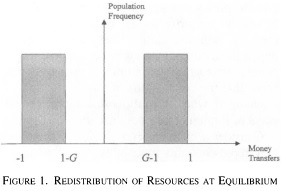
\includegraphics[scale=0.75]{distribution.jpg}
\end{center}
\end{figure}

\noindent Intuitively: to beat the utility that each voter would have with $G$, an optimal schedule transfer entails giving more than $G-1$ to some voters and ``taxing'' the others.

\bigskip

\noindent We have a more unequal distribution the higher is $G$: need to take a lot from the ``unlucky'' voters to buy the ``lucky'' ones.
\end{frame}


\begin{frame}
\frametitle{Intuition for probability of providing $G$}
\noindent In equilibrium we have:
\begin{itemize}
\item FPTP: probability of providing $G$ is $\frac{1}{2}$, independent of the value of $G$.
\item FPTP: probability of providing $G$ is $G-1$, increasing in value of $G$.
\end{itemize}

\bigskip

\noindent Why? Need to think about best possible deviations.

\end{frame}

\begin{frame}
\frametitle{Intuition for probability of providing $G$}
\noindent Deviation from the mixing equilibrium can be done in two ways:
\begin{itemize}
\item If the opponent ends up providing the public good, \textit{ex ante}, in the best deviation, I need to offer a little more than $G-1$ to win voters:
\begin{itemize}
\item PR: I will offer a little more than $G-1$ to a little less than $\frac{1}{G}$.
\item FPTP: always possible to win a majority of voters, I don't care about size of majority. 
\end{itemize}
\item If the opponent ends up providing transfers, \textit{ex ante}, in the best deviation, I want to take from voters getting positive transfers and buy as many ``cheap'' voters as possible. 
\begin{itemize}
\item PR: I can buy more ``unlucky'' voters the higher $G$, since the ``lucky'' voters that I am taxing were getting a higher transfer by the other candidate.
\item FPTP: again, I don't care about size of majority: always possible to win a majority.
\end{itemize}
\end{itemize}

\end{frame}



\begin{frame}
\frametitle{Intuition for probability of providing $G$}
\noindent Therefore:
\begin{itemize}
\item FPTP:  I am ex ante indifferent between the two types of deviations: I just need 50 percent of the votes, and that is always possible. Therefore to discourage both kind of deviations we need an equal likelihood that the opponent offers public good or transfers, independently of G.
\item PR: the higher $G$, the less votes I can get if I choose the best deviation if the opponent ends up providing $G$, and the more those that I can get if I choose the best deviation if the opponent ends up providing transfers: to avoid both deviations simultaneously, the probability that the opponent provides $G$ must increase with the size of $G$
\end{itemize}
\end{frame}

\begin{frame}{Implications?}

\begin{tcolorbox}
What are the testable implications of these results?
\end{tcolorbox}

\pause 

\begin{tcolorbox}
What's missing from the model?
\end{tcolorbox}
\end{frame}

\begin{frame}{What's missing: political coalitions? }

\begin{figure}
\centering
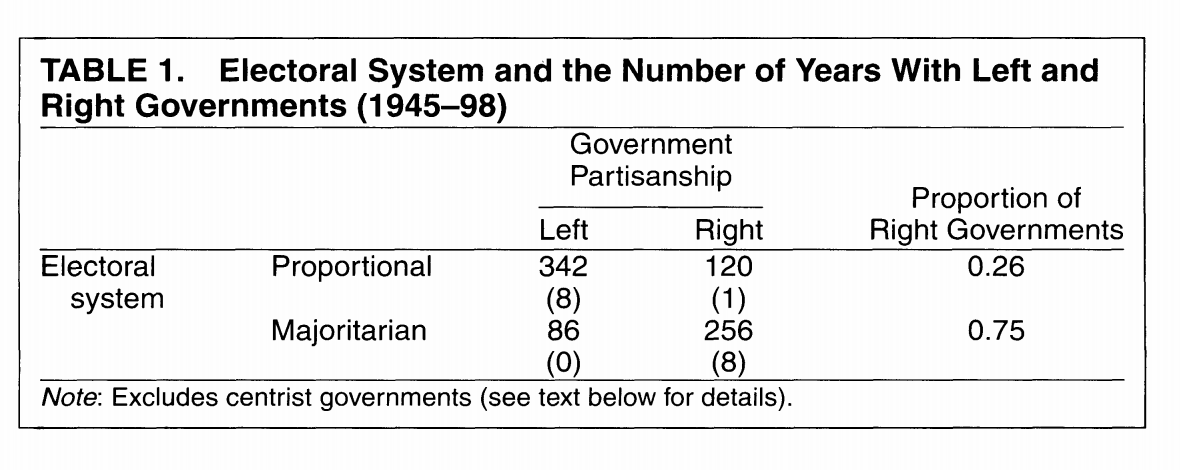
\includegraphics[width=\textwidth]{iversen.png}
\end{figure}

\vspace{-1em}
\footnotesize Iversen, Torben, and David Soskice. ``Electoral institutions and the politics of coalitions: Why some democracies redistribute more than others.'' \textit{American Political Science Review} 100.2 (2006): 165-181.

\end{frame}

%\textbf{EDIT: Under PR, candidates max vote share -- margin of victory of the redistributive plan vs. public good falls as public good becomes more valuable. Reduction in number of voters to whom a candidate can promise benefits that are worth more than the benefits provided by public good. FPTP -- attractiveness of redistribution does not depend on value of $G$.}

\begin{frame}
\frametitle{Persson, Roland \& Tabellini (2000)}

Huge variation in size and composition of government spending over time and across countries.

\begin{itemize}
\item PRT: aim to provide a micro-founded public finance model of government outputs in different political systems. 
\item Parliamentary vs presidential $\rightarrow$ differences in collective decisions on taxation, redistribution, public goods, rents.
\end{itemize}

\bigskip

\noindent Foundational principles:

\begin{itemize}
\item People are selfish.
\item Policy delegation by electors (principals) to  representatives (agents): no direct democracy.
\item No outside enforcement $\rightarrow$ no commitment.
\end{itemize}

\bigskip

\noindent A typical agency problem: how can voters get politicians to act as they want? 

\end{frame}


\begin{frame}
\frametitle{Persson, Roland \& Tabellini (2000)}

PRT focus on the implications of these three assumptions under different political systems. Useful to contrast to models we've looked at in this class:

\begin{itemize}
\item Downs (1957), Lindbeck \& Weibull (1987): Ignores commitment.
\item Besley \& Coate (1997): Rules out the agency problem.
\item Barro (1973), Ferejohn (1986): Ignores institutions.
\item Meltzer \& Richard (1987): Ignores delegation.
\end{itemize}

\bigskip

Political process $\rightarrow$ taxes, public goods, rents. Three conflicts:
\begin{itemize}
\item Politicians taking rents from voters.
\item Voters disagreeing over allocation of tax revenues.
\item Politicians disagreeing over distribution of current/future rents.
\end{itemize}

\end{frame}


\begin{frame}\frametitle{Persson, Roland \& Tabellini (2000)}

Political constitutions like an incomplete contract: specifies decision-making process. Key variation in \textit{separation of powers} and \textit{legislative cohesion}.

\begin{itemize}
\item Presidential: separation of powers $\rightarrow$ less scope for collusion between politicians (so less agency problem). Smaller government, inefficiently small spending on public goods.
\item Parliamentary: larger government, more redistribution which benefits a broader set of voters due to more legislative cohesion (solves conflict between voters).
\end{itemize}

\end{frame}


\begin{frame}
\frametitle{Setup}

\noindent Infinite number of periods $t$.  Policy vector $\textbf{q}_t = (\tau_t, g_t, \textbf{r}_t^i, \textbf{s}_t^l)$ chosen every period.
\begin{itemize}
\item $\tau$ common lump sum tax, $r^i_t$ transfers to group $i$, $g_t$ public good, $\textbf{s}_t$ rents to incumbent $l$.
\end{itemize}

\noindent \textbf{Voters}: three internally homogeneous geographic groups $i=\{1,2,3\}$ each with population mass 1 (indirect) utility/preferences in period $j$: 

$$u_j^i=\sum_{t=j}^{\infty} \delta^{t-j}U^i(\textbf{q}_t)$$ 

where $\delta <1$ is a discount factor common to all actors  and $$U^i(\textbf{q}_t) = c^i_t + H(g_t) = 1-\tau_t + r_t^i + H(g_t)$$ with $H'>0$, $H''<0$ and $H'(0)>1$.
\end{frame}

\begin{frame}
\frametitle{Setup}

\noindent \textbf{Politicians}: infinite potential politicians, always three incumbents $l$ who maximize the discounted present value of their rents: 

$$v_t^l = \sum_{t=j}^{\infty} \delta^{t-j} s_t^l D^l_t$$

$D^l_t = \{0,1\}$ is an indicator for whether $l$ holds office in period $t$. A politician can never return to office. Note that rents have different values for different politicians (but we abstract from that). 

%\bigskip

%Note that contractual incompleteness $\rightarrow$ rents in equilibrium.

%\noindent In these models: The citizens can constrain their representative to get no more rents than up to the point in which politician is indifferent between behaving and deviating (i.e. set maximum tax and appropriate everything, being then send home..)


\end{frame}


\begin{frame}
\frametitle{Setup}

\noindent Government budget constraint is: 

$$3\tau_t = \sum_i r_t^i + \sum_l s_t^l + g_t$$  

so there are no waste or work disincentives.

\bigskip 

Constitution will affect the balance between:
\begin{itemize}
\item Activities benefitting all $i$: $g_t$, $-\tau_t$.
\item Activities benefitting some $i$: $\textbf{r}_t^i$.
\item Activities benefitting some $l$: $\textbf{s}_t^l$.
\end{itemize}

\end{frame}



\begin{frame}
\frametitle{Initial benchmarks}

\noindent \textbf{Social Planner}: sets $$\textbf{q}_t = \arg \max_{\textbf{q}_t} \sum_i U^i(\textbf{q}_t)$$  which yields $s_t^l=0, \forall l$ and $r_t^i=0, \forall i$.

Set $g_t$ to maximise $3[1-\tau_t + H(g_t)] \Rightarrow g_t = H'^{-1}(\frac{1}{3})$ and $\tau_t=\frac{H'^{-1}(\frac{1}{3})}{3}$.

\bigskip

\noindent \textbf{Leviathan}: sets $s_t^{Lev}=3$ and $\tau_t=1$ in any given period.

\end{frame}

\begin{frame}
\frametitle{A simple legislature}

%\noindent First consider a simple legislative bargaining model (simplified Baron \& Ferejohn 1989) with no policy commitment and retrospective punishment (a la Baron 1973, Ferejohn 1986) in a plurality electoral system. 

\noindent Sequence of play for any period $t$:

\begin{enumerate}
\item Nature selects agenda-setter $a$ from $l=1,2,3$ w.p. $p_l=\frac{1}{3}$. 

\item All voter groups $i$ choose and reveal optimal re-election rules $b_t^i|a$. 

\item $a$ proposes $\textbf{q}_t$

\item All $l$ vote under majority rule -- if 2 are in support it passes, otherwise bargaining ends with status quo policy $\tau_t=s^l_t=\sigma >0, \forall l$ and $g_t=r^i_t=0, \forall i$. (A sad status quo)

\item All $i$ vote on whether to keep their corresponding $l$ in office according to re-election rule.
\end{enumerate}

\end{frame}

\begin{frame}
\frametitle{A simple legislature}

\begin{figure}[h]
\begin{center}
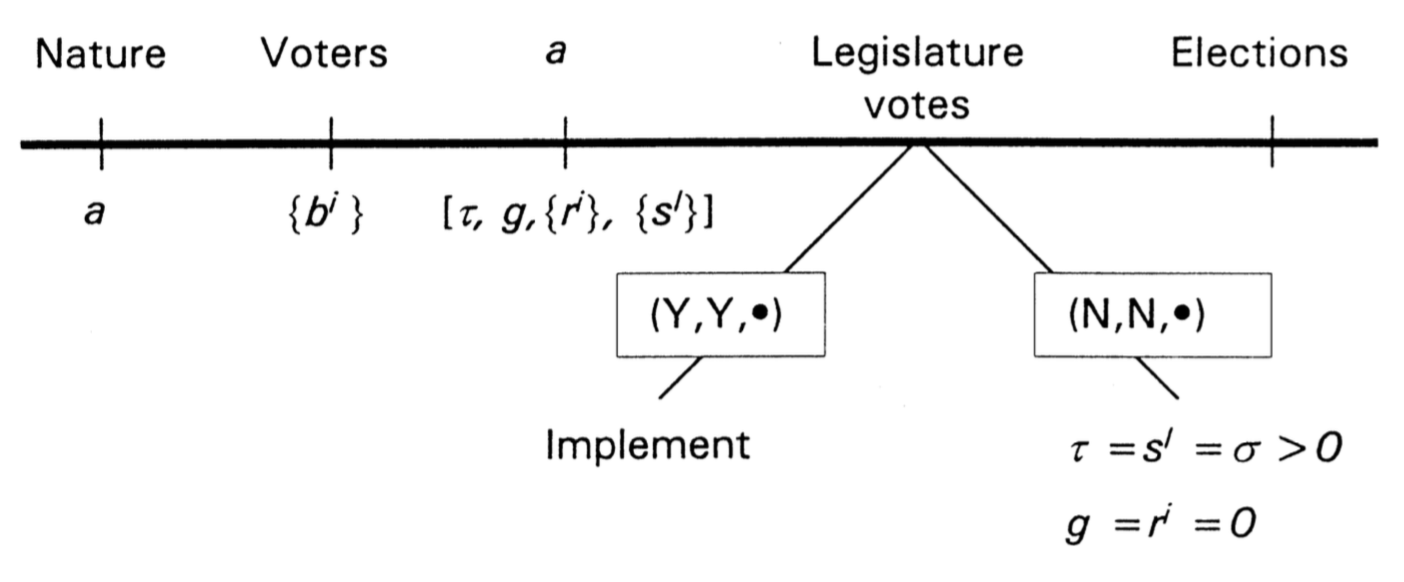
\includegraphics[scale=0.4]{PRT.png}
\end{center}
\end{figure}

\end{frame}



\begin{frame}
\frametitle{Voting rule}

\noindent Voters in each district choose the following rule, conditional on whether $i=a$ (which they observe): 

$$D^l_{t+1} = 1 \text{ if } U^i(\textbf{q}_t) \geq b_t^i$$ 

which yields a vector of each $i$'s reservation values $\textbf{b}_t$ (known to politicians) for $i = a$ and $i \neq a$.

%\bigskip

%Since agenda-setters will have power, it makes sense that the reservation utility will be different for them.

\end{frame}

\begin{frame}
\frametitle{Equilibrium concept}

\noindent There are many equilibria -- so let's keep things simple-ish.

\begin{itemize}
\item Voters \textit{across} constituencies do not coordinate.

\item Stationary strategies.% (i.e. voters cannot commit to strategies over elections).
\end{itemize}

So voters cooperate within districts but play Nash against others.

\medskip

\noindent Three criteria define a unique stationary equilibrium $\textbf{q}^L_t(\textbf{b}^L_t)$ and reservation utilities $\textbf{b}^L_t$:

\begin{enumerate}
\item $\forall \textbf{b}_t, \exists i \neq a$ such that $i$ prefers $\textbf{q}^L_t(\textbf{b}^L_t)$ to the reversion outcome.

\item $a$ prefers $\textbf{q}^L_t(\textbf{b}^L_t)$ to any other outcome satisfying point 1.

\item $\forall i, b_t^{iL}$ is optimal given $\textbf{q}^L_t(\textbf{b}^L_t)$ and $b_t^{-iL}$.
\end{enumerate}


\end{frame}

\begin{frame}
\frametitle{Results in simple legislative game}

\noindent \textbf{Proposition 1}

\noindent In equilibrium in the simple $L$ game we have 

\vspace{-0.5cm}

\begin{align*}
\tau^L&=1 \\
s^L&=3\frac{1-\delta}{1-(\delta/3)} \\
g^L&=\min \left[ \hat{g},\frac{2\delta}{1-(\delta/3)} \right]
\end{align*}

where $\hat{g}$ is implicitly defined by $H'(\hat{g})=1$.

\vspace{-0.5cm}

\begin{align*}
r^{aL}&=\frac{2\delta}{1-(\delta/3)}-g^L\geq 0 \\
r^{iL}&=0, \forall i\neq a \\
b^{aL}&=H(g^l)-g^L+\frac{2\delta}{1-(\delta/3)} \\
b^{iL}&=H(g^L), \forall i\neq a
\end{align*}

\end{frame}


\begin{frame}\frametitle{Results in simple legislative game}

...and all politicians get reelected. So taxes are maximal, $g$ underprovided, some redistribution goes to a minority, and legislators get rents.

\bigskip

\textbf{A.} Bertrand competition between districts.

\begin{enumerate}
\item Consider $m, n \neq a$.
\item $a$ only needs support of one other legislator.
\item If $n$ is excluded, then $s^n = r^n = 0$.
\item So district included will be the cheapest one -- depends only on $b^n$ and $b^m$.
\item Implies Bertrand competition for transfers between voters of different districts -- so $r^m = r^n = 0$, and $b^m = b^n = 1-\tau+H(g)$.
\end{enumerate}

\end{frame}


\begin{frame}
\frametitle{Results in simple legislative game}

\textbf{B.} Legislators get re-elected. 

\begin{enumerate}
\item $W$ expected equilibrium continuation value before Nature.
\item Consider legislator $m$: if $a$ wants re-election, will never offer more than:
$$ s^m = \sigma - \delta W$$
\item This leaves $m$ indifferent between voting yes and getting reappointed, and voting no, getting $\sigma$, then losing office.
\item If $a$ does not want re-election, will just offer $\sigma$ to $m$ to win support, then $g=r=0$ and $\tau=1$.
\item So $a$ seeks re-election $\Leftrightarrow s^a + \delta W \geq 3 - \sigma$.
\item So $a$ and $m$ implement policies leading to re-election $\Leftrightarrow s = s^m + s^a \geq 3 - 2\delta W$.
\item Since $r = 0$ in $m, n$, reservation utility of voters the same $\rightarrow$ both get re-elected.
\end{enumerate}

\end{frame}

\begin{frame}{Results in simple legislative game}

\textbf{B.} Legislators get re-elected. (cont'd)

$a$ wants to minimise payment to $m$ and satisfy re-election constraints in $a$ and $m$ with equality -- and take the rest for themselves. So wants to set $\tau = 1$ if they can.

\end{frame}

\begin{frame}\frametitle{Proving Proposition 1}

\begin{enumerate}
\item Consider voters in $a$. We know $r^a = r$.
\item Policy maximising their utility is argmax $(r + 1 - \tau + H(g))$ subject to government budget constraint and politician IC constraint.
\item Combining constraints: $3(\tau - 1) + 2\delta W \geq r + g$.
\item Solution implies $\tau = 1$, $g = \text{min}(\hat{g}, 2\delta W)$, $r = 2\delta W - g$, $s = 3 - 2\delta W$. 
\item All legislators are reappointed, which implies $W = \frac{s}{3} + \delta W$.
\end{enumerate}

This gets us to the equilibrium (Proposition 1) by substituting in.

\end{frame}

\begin{frame}
\frametitle{Intuition for results:}
\noindent Voters in $m, n$ compete a la Bertrand for transfers: so they get 0 transfer.

\medskip

\noindent Voters in $a$ discipline agenda setter: minimum rent to have incentive to be re-elected. Also other legislators get re-elected, given that their voters, being rational, lower the standards to re-elect them.

\medskip

\noindent  Voters in $a$'s district are the only to get transfers, so they prefer maximum taxation. %and they cause under provision of public good since they trade off redistribution and public good one for one.

\medskip

\noindent Agenda-setter is basically just setting policy to maximise the utility of voters in $a$. In conclusion: wasteful rents, under-provision of public good, and politically powerful minority receive all redistribution.  
\end{frame}


\begin{frame}
\frametitle{Characterizing presidential systems}

\noindent Defining feature for PRT is separation of powers: capture this with distinct agenda-setters on the budget and spending. 

\bigskip

\noindent Key idea: separation of powers exploits conflict between politicians to reduce the agency problem.

\end{frame}

\begin{frame}
\frametitle{Presidential ($C$) system}

\begin{enumerate}
\item Nature randomly selects $a_{\tau}$ and $a_g$ (where no $l$ can be both). (So $l\in\{a_\tau, a_g, n\}.$)

\item All voter groups $i$ choose and reveal optimal re-election rules $b^i|a_{\tau},a_g,n$. 

\item $a_{\tau}$ proposes budget $\tau$. 

\item All $l$ vote on $\tau$ under majority rule -- if 2 are in support it passes, otherwise bargaining ends with status quo policy $\tau=\sigma <1$. 

\item $a_g$ proposes spending $\{g,\textbf{s},\textbf{r}\}$ subject to budget constraint $\sum_i r^i+\sum_l s^l+g \leq 3\tau$
\item All $l$ vote on $\{g,\textbf{s},\textbf{r}\}$ under majority rule -- if 2 are in support it passes, otherwise bargaining ends with status quo policy $s^l=\tau, \forall l$ and $g=r^i=0, \forall i$.

\item All $i$ vote on whether to keep their corresponding $l$ in office according to re-election rule $b^i|a_{\tau},a_g,n$.
\end{enumerate}

\end{frame}


\begin{frame}
\frametitle{Presidential ($C$) system}

\begin{figure}[h]
\begin{center}
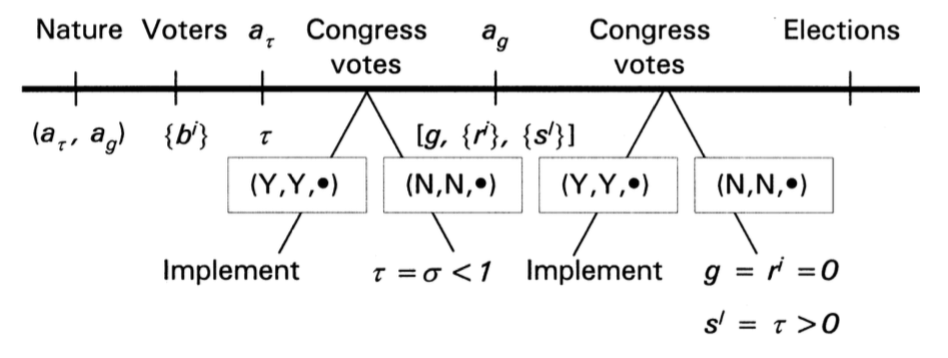
\includegraphics[scale=0.5]{PRT_pres.png}
\end{center}
\end{figure}

\end{frame}




\begin{frame}
\frametitle{Solution to the presidential game}

\footnotesize
\noindent \textbf{Proposition 2}

\noindent In equilibrium in the presidential game $C$ we have $$\tau^C=\frac{1-(\delta/3)}{1+(2\delta/3)}<\tau^L=1$$ $$s^C=3\frac{1-\delta}{1+(2\delta/3)}<s^L$$ $$g^C=\min \left[ \hat{g},\frac{2\delta}{1+(2\delta/3)} \right] \leq g^L$$ where $\hat{g}$ is implicitly defined by $H'(\hat{g})=1$ $$r^{a_g C}=\frac{2\delta}{1+(2\delta/3)}-g^C\leq r^{aL}$$ $$r^{iC}=0, \forall i\neq a$$ $$b^{aC}=H(g^C)-g^C+\frac{2\delta}{1+(2\delta/3)}$$ $$b^{iC}=H(g^C), \forall i\neq a$$

\end{frame}

\begin{frame}
\frametitle{Intuition for the result:}

Solve the game through backward induction:

\begin{enumerate}
\item In last stages, voters of districts other than $a_g$ again compete Bertrand-style and get no transfers.
\item Voters in $a_t$ -- seeing what will happen -- set taxes to minimum such that their legislator behaves. 
\item Public goods even lower -- since $W$ is lower -- than in $L$. 
\item Government waste is lower because $a_g$ has access to less revenue, so IC constraint faced by voters is less severe.
\end{enumerate}

\end{frame}

\begin{frame}{Presidential regime: Observations}

\noindent Separation of powers produces lower taxes, redistribution to powerful minority, and rents: smaller size of government.

\medskip

\noindent But we need separation of powers over \textbf{size} and \textbf{division} of the pie to have check and balances.

\medskip

\noindent Interpretation: Presidential-Congressional regime as in the US, with:
\begin{itemize}
\item Different committees with proposal power over different policy dimensions;
\item No need of forming stable coalitions to support the executive (since directly elected): low legislative cohesion. 
\end{itemize}
\end{frame}


\begin{frame}
\frametitle{Parliamentary ($P$) systems}

\noindent Parliamentary systems characterized by random members of a legislative coalition making up the ``government''. One member is senior and proposes a budget. 

\medskip

The intuition is that legislators are tied together by legislative power relative to being out of the governing coalition, but senior coalition partner has more power. 

\bigskip

If junior coalition member opposes proposal, she causes a crisis: instead of leading to the status quo (as in presidential regime), this leads to a new agenda setter chosen.

\end{frame}

\begin{frame}
\frametitle{Game play in parliamentary systems}

\begin{enumerate}
\item Nature randomly selects a senior coalition partner $a$ and a junior coalition partner $m$.

\item All voter group $i$ choose and reveal optimal re-election rules $b^i|a,m$.

\item $a$ proposes $\textbf{q}_a$ subject to the budget constraint $\sum_i r_a^i + \sum_l s_a^l + g_a \leq 3 \tau$.

\item $m$ then gets to choose whether to veto $\textbf{q}_a$: if not, it passes and we then proceed to elections; if vetoed, move to the next stage...

\item Play the simple legislative bargaining game with $a^{\prime}$ now randomly selected from $i=\{a, m, n\}$ (voters recalibrate to $b^l|a^{\prime}$)

\item All $i$ vote on whether to keep their corresponding $l$ in office according to re-election rule $b^i|a_{\tau},a_g$.
\end{enumerate}

\end{frame}


\begin{frame}
\frametitle{Parliamentary ($P$) system}

\begin{figure}[h]
\begin{center}
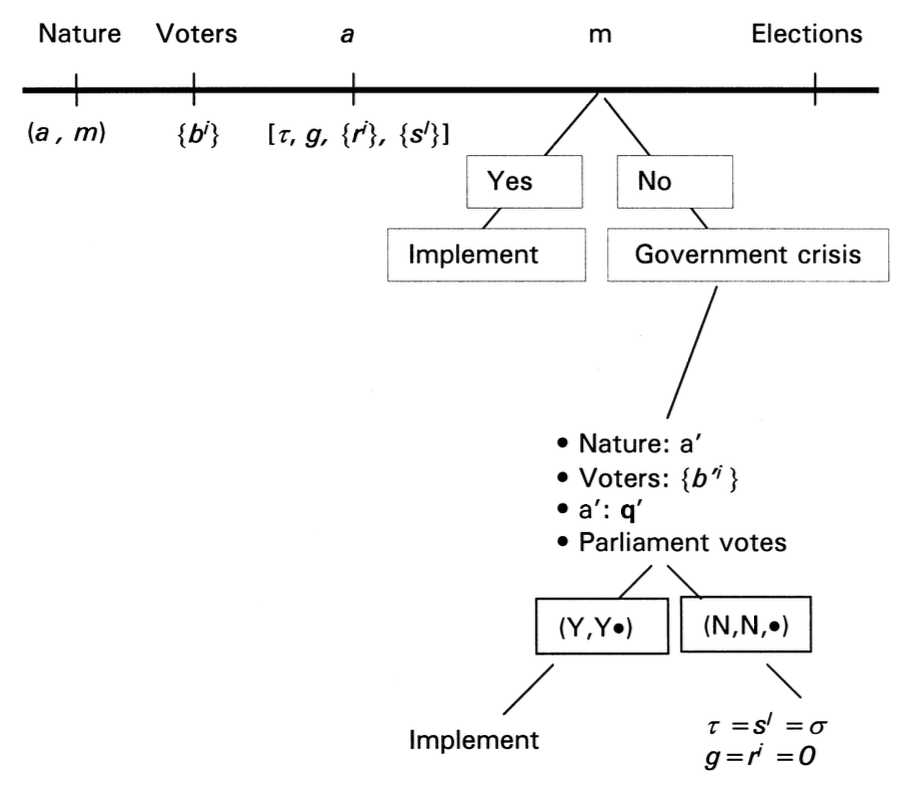
\includegraphics[scale=0.5]{PRT_parl.png}
\end{center}
\end{figure}

\end{frame}





\begin{frame}
\frametitle{Solution to the parliamentary game}

\noindent \textbf{Proposition 3}

\noindent In equilibrium in the parliamentary game $P$ we have a continuum of equilibria: $$\tau^P=1=\tau^L>\tau^C$$ $$s^P=3\frac{1-\delta}{1-(\delta/3)}=s^L>s^C \text{ with } s^{aP}=\frac{2}{3}s^P, s^{mP}=\frac{1}{3}s^P$$ $$\bar{g} \geq g^P>g^C \text{ where } H'(\bar{g})=\frac{1}{2}$$ $$r^P=\frac{2\delta}{1-(\delta/3)}-g^P \geq 0, \forall i\neq n \text{ where } g^P=\bar{g} \;\; \text{if} \;\; r^{iP}>0 \text{ for } i=a,m$$ $$b^{iP}=H(g^P)+r^{iP} \text{ or } b^{a'P} = H(g')-g'+\frac{2\delta}{1-(\delta/3)}$$ $$b'=H(g') \text{ with } g'=\min \left[ \hat{g},\frac{2\delta}{1-(\delta/3)} \right]$$

\end{frame}

\begin{frame}
\frametitle{Intuition for the result}

\noindent $a$ and $m$ have veto rights: voters in their districts can demand higher transfers: bilateral monopoly replaces Bertrand competition for transfers.%\\
%Mutually compatible transfers' requests can take several forms, so we have a multiplicity of equilibria.

\noindent Higher taxation than in Presidential regime, and redistribution from minority to majority.

\noindent Public good provision higher, since benefit of the public good now internalised by two districts instead of one -- but given the desirability of transfers at the expense of the minority, still under provision relative to optimum.

\end{frame}


\begin{frame}
\frametitle{Intuition for the result}

\noindent The threat of going through a government crisis now enables legislators to appropriate as much rents as in the simple legislature game, but now rents are more equally distributed.

\bigskip

Why? Voters know that, if there is a government crisis, there is a new process of government formation (with rents given by $L$): this threat allows the government coalition to extract more rents.

\end{frame}

\begin{frame}
\frametitle{Comparing utility: an inevitable trade-off?}

\noindent The difference in expected utility between the systems is $$E(u^{iP})-E(u^{iC}) = $$ $$\frac{1}{1-\delta} \left( H(g^P)-\frac{1}{3}g^P - [H(g^C)-\frac{1}{3}g^C] - \frac{\delta(1-\delta)}{(1-(\delta/3))(1+(2\delta/3))} \right)$$ where the first two terms give the relative benefit from $G$ closer to optimum in $P$, but the third term captures the deadweight loss associated with higher $s$ in $P$.

\end{frame}

\begin{frame}
\frametitle{Conclusions}


\begin{itemize}
\item Parliamentary regimes $\rightarrow$ larger govt vs persidential regimes
\item $P$ better for voters when $g^P > g^C$ or if $\delta$ small.
\item $P$ also gives greater equality of transfers.
\item PRT show some empirics on government size being larger in $P$. (One estimate: spending in presidential-congressional regimes lower by 10\% of GDP versus parliamentary!)
\item Endogenous institutional choice? $s$ higher under $P$ so constitution-writers should not have electoral incentives.
\end{itemize}

\end{frame}

\begin{frame}{Trade-offs}

``The parliamentary regime appears better for voters if the underprovision problem is great (because public goods are very valuable), whereas the presidential regime dominates if the political agency problem is highly relevant (because politicians face small transaction costs in rent extraction or the punishment from losing the next election is small - for instance, because of barriers to entry in the political arena).'' (PT p.267)

\end{frame}

\begin{frame}{Discussion q's}

\begin{tcolorbox}
Does the model capture the key features of parliamentary vs presidential regimes?
\end{tcolorbox}

\vspace{3em}
\begin{tcolorbox}
How convincing are their empirics?
\end{tcolorbox}

\end{frame}

\end{document}
